\section{Evaluation}
Due to a misunderstanding, the custom generator for the evaluation-part, started out as a custom generator for the training and validation data. Since a lot of work was put into this, it will be briefly described as well. The directories was split into training and validation data by creating a new database, that contained two subsets; A training set with $1072$ samples of each class and a validation set with $269$ samples of each class.  The structure is as follows: 
\newline
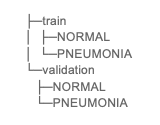
\includegraphics[scale=0.5]{dir}
\newline
\newline
Before beginning the datagenerator for the training data, there was made a label and partition dictionary with the paths for the images. The images' labels was encoded as $0$ for normal and $1$ for pneumonia. The datagenerator has a function, that loads the images in grayscale format to change the colorchannels from $3$ to $1$. The datagenerator also rescales the values of every pixel to between $0$ and $1$, since this is often improving performance of a neural net. 
\newline
\newline
\textbf{The Custom Data-Generator}
\newline
A data-generator is conceptually simple. It is a stream of input, through a filter or transformation, to a desired output.
For this generator specifically, the goal was to have it read the matrix of values from the .txt correctly and output it in a way, that the model could interpret. The datagenerator takes the directory as an input, together with specifications of the image-size. The generator makes a list of files and creates a list of labels determined by which directory the file comes from. The generator then needed a function to convert the txt-file to a more image-like file for the model to read. The generator has the function convert,  that takes a batch of files as input. It starts by creating empty arrays to store the values and labels in..  Then it goes through the batch, reads the values from the txt-file, rescales it to normalized values like in the training-data, reshapes the values and appends the values and labels to the empty arrays. It finally returns the batch of values and labels. Through the testing, it turns out, that for now, the generator only works with a batch-size of $1$, but for this purpose it will do. If the generator was supposed to be for the training part, it would need a little more work.  